\chapter{A brief tour of OTB-Applications}\label{chap:otb-applications}

\section{Introduction}\label{sec:appintro}

\app was perhaps the older package of the \otb suite after the OTB
package itself. Since the \otb is a library providing remote sensing
functionalities, the only applications that were distributed at the
beginning were the examples from the Software Guide and the
tests. These applications are very useful for the developer because
their code is very short and only demonstrates one functionality at a
time. In many cases, a real application would require :
\begin{itemize}
\item combining together two or more functions from the \otb
\item providing a nice high level interface to handle : parameters, input data,
output data and communication with the user
\end{itemize}

The \app package was originally designed to provide applications
performing simple remote sensing tasks, more complex than simple
examples from the Software Guide, and with a more user-friendly
interface (either graphical or command-line), to demonstrate the use
of the \otb functions. The most popular applications are maybe the
\application{otbImageViewerManager}, which allows to open a collection
of images and navigate in them, and the
\application{otbSupervisedClassificationApplication}, which allowed to
delineate training regions of interest on the image and classify the
image with a SVM classifier trained with these regions (this
application is no longer maintained since the same functionnality is
available through the corresponding \mont module). During the first 3
years of the \otb development, many more applications have been added
to this package, to perform various tasks. Most of them came with a
graphical user interface, apart from some small utilities that are
command-line.

The development and release of the \mont software (see
chapter~\ref{chap:Monteverdi} at the end of year 2009 changed a lot of
things for the \app package: most of non-developer users were looking
for quite a long time for an application providing \otb
functionalities under a unified graphical interface. Many applications
from the \app package were integrated to \mont as modules, and the
\app package lost a lot of its usefulness. No more applications were
added to the package and it was barely maintained, as new graphical
tools were directly embedded within \mont.

Then, some people started to regain interest in the \app
package. \mont is a great tool to perform numerous remote sensing and
image processing task in a minute, but it is not well adapted to
heavier (and longer) processing, scripting and batch
processing. Therefore, in 2010 the \app package has been revamped: old
applications have been moved to a legacy folder for backward
compatibility, and the development team started to populate the
package with compact command-line tools to perform various heavy
processing tasks. 

Later on in 2011, the \app has been further revamped. Because of the
increasing need to interface the \app into other software and to
provide auto-generated interfaces, the \otb development team decided
to develop a new application framework. The main idea of this
framework is the following: each application is written once for all
in a shared library (also known as plugin). This plugin can be
auto-loaded into appropriate tools wihtout recompiling, and is able to
fully describe its parameters, behaviour and documentation.

The tools to use the plugins can be extended, but \otb shipped the
following:
\begin{itemize}
\item A command-line laucher, which is almost equivalent to the former
  \app command-line interface,
\item A graphical launcher, with an auto-generated QT interface,
  providing ergonomic parameters setting, display of documentation,
  and progress reporting,
\item A SWIG interface, which means that any application can be
  loaded set-up and executed into a high-level language such as Python
  or Java for instance.
\end{itemize}

Additionally, \href{http://www.qgis.org/}{QGis} plugins built on top of the SWIG/Python interface
are available with seamless integration within QGis. You can find a short guide about it \href{http://wiki.orfeo-toolbox.org/index.php/Quantum_GIS_access_to_OTB_applications}{here}.

To facilitate the use of these tools and applications, they will now
be shipped with the standard \otb package. It means that the former
\textbf{OTB-Applications} package has entered its maintenance cycle :
no new feature will be pushed there, and all development is done directly
inside the \otb paackage.

The \app are now rich of more than 40 tools, which are listed in the
the applications reference documentation, presented in
chapter~\ref{chap:apprefdoc}, page~\pageref{chap:apprefdoc}.

\section{Installation}\label{sec:appinstall}

We provide different standalone binary packages for OTB-Applications:
\begin{itemize}
\item for Windows platform (Seven and later)
\item for 64bit Linux distribution
\item for MacOS X
\end{itemize}

Other binaries can be available as packages (OSGeo packages, Debian/Ubuntu packages,
OpenSuse packages), however be advised that they may not be up-to-date nor delivered
with full features.
If you want to build from source or if we don't provide packages for your system,
some informations are available into the \sg, in the section \textbf(Building from Source)

\subsection{Windows}

We provide \app for Windows Seven and later through standalone packages.
They are cross-compiled with MinGW, for 32bit and 64bit platforms.
They contain all \app and their launchers (both command line and graphical
launchers are provided). Check the download page :
\href{https://www.orfeo-toolbox.org/download}{OTB Download page}

There is a 32bit and a 64bit version. They contain the same directory structure:
\begin{itemize}
\item \verb?monteverdi.bat? : A launcher script for \mont
\item \verb?mapla.bat? : A launcher script for Mapla
\item \verb?otbenv.bat? : A script to initialize the environment for OTB executables
\item \verb?bin? : A folder containing application launchers (otbcli\textunderscore *.bat,
otbgui\textunderscore *.bat) and the DLLs.
\item \verb?lib? : A folder containing application DLLs.
\end{itemize}

The applications can be launched from the Mapla launcher. If you want to use
the otbcli and otbgui launchers, you should before initialize a command prompt
with \verb?otbenv.bat?. 

\subsection{Linux 64bit}

We provide \app for Linux 64bit OS through standalone packages.
They contain all OTB Applications and their launchers (both command line and graphical
launchers are provided). Check the download page :
\href{https://www.orfeo-toolbox.org/download}{OTB Download page}

This package is a self-extractible archive. You may uncompress it with a
double-click on the file, or with the command line :
\begin{verbatim}
> sh  OTB-5.2.1-Linux64.run
\end{verbatim}

Please note that the resulting installation is not meant to be moved, you should
uncompress the archive in its final location. Once the archive is extracted, 
the directory structure is made of :
\begin{itemize}
\item \verb?monteverdi.sh? : A launcher script for \mont
\item \verb?mapla.sh? : A launcher script for Mapla
\item \verb?otbenv.profile? : A script to initialize the environment for OTB executables
\item \verb?bin? : A folder containing application launchers (otbcli\textunderscore *.sh,
otbgui\textunderscore *.sh), Monteverdi and Mapla.
\item \verb?lib? : A folder containing all shared libraries and OTB applications.
\item \verb?share? : A folder containing common resources and copyright mentions.
\end{itemize}

In order to run the command line launchers, this package doesn't require any special
library that is not present in most modern Linux distributions. The graphical
executable (otbgui launchers, Monteverdi and Mapla) use the X11 libraries, which
are widely used in a lot of distributions :
\begin{verbatim}
libx11-6 libxext6 libxau6 libxxf86vm1 libxdmcp6 libdrm2
\end{verbatim}
Monteverdi also requires the standard graphics libraries \textbf{libgl1} and
\textbf{libglu1}. Make sure you have at least one version of them installed in
your system.

The applications can be launched from the Mapla launcher. If you want to use
the otbcli and otbgui launchers, you should before initialize your environment
with \verb?otbenv.profile?.

\subsection{MacOS X}

We provide \app for MacOS X through a standalone package. This package is a 
self-extractible archive, quite similar to the Linux one. You may uncompress 
it with the command line :
\begin{verbatim}
> sh  OTB-5.4.0-Darwin64.run
\end{verbatim}

Please note that the resulting installation is not meant to be moved, you should
uncompress the archive in its final location.

Once the archive is extracted, the directory structure is made of :
\begin{itemize}
\item \verb?monteverdi.sh? : A launcher script for \mont
\item \verb?mapla.sh? : A launcher script for Mapla
\item \verb?otbenv.profile? : A script to initialize the environment for OTB executables
\item \verb?bin? : A folder containing application launchers (otbcli\textunderscore *.sh,
otbgui\textunderscore *.sh), Monteverdi and Mapla.
\item \verb?lib? : A folder containing all shared libraries and OTB applications.
\item \verb?share? : A folder containing common resources and copyright mentions.
\end{itemize}

The applications can be launched from the Mapla launcher. If you want to use
the otbcli and otbgui launchers, you should before initialize your environment
with \verb?otbenv.profile?.

\subsection{Other packages}

\textbf{Warning !} These packages may not be up-to-date with latest OTB releases.
In addition, some features of the library may not be available on every platform.
Some of these are not maintained by the OTB-team. If you want to get involved in
the packaging of OTB for your platform, please contact us through the developer's
mailing list :
\href{mailto:otb-developers@googlegroups.com}{otb-developers@googlegroups.com}.

\subsubsection{OSGeo4W}

Since version 3.12, we provide \app packages through OSGeo4W for Windows XP/Seven users:
\begin{itemize}
\item \textbf{otb-bin} for command line and QT applications
\item \textbf{otb-python} for python applications
\end{itemize}
Follow the instructions in the installer and select the packages you want to add. The installer will proceed with the installation of selected packages and all their dependencies.
For the \textbf{otb-bin} packages, it will be available directly in the OSGeo4W shell, for example run
\begin{verbatim}
otbgui_BandMath.
\end{verbatim}
For the \textbf{otb-python} packages, you can simply check from an OSGeo4W shell the list of available applications:
\begin{verbatim}
python
import otbApplication
print str( otbApplication.Registry.GetAvailableApplications() )
\end{verbatim}

\subsubsection{Debian}

There are OTB packages for Debian (unstable) since version 5.2.0.
OTB Applications packages may be available as
Debian packages through APT repositories:
\begin{itemize}
\item \textbf{otb-bin} for command line applications
\item \textbf{otb-bin-qt} for Qt applications
\item \textbf{python-otb} for python applications
\end{itemize}

Due to license issues, the OTB package built in Debian doesn't contain 6S. As
a consequence, the package does not contain the OpticalCalibration application.

\subsubsection{Ubuntu 12.04 and higher}

For Ubuntu 12.04 and higher, OTB Applications packages may be available as
Debian packages through APT repositories:
\begin{itemize}
\item \textbf{otb-bin} for command line applications
\item \textbf{otb-bin-qt} for Qt applications
\item \textbf{python-otb} for python applications
\end{itemize}

Since release 3.14.1, OTB Applications packages are available in the
\href{https://launchpad.net/~ubuntugis/+archive/ubuntugis-unstable}{ubuntugis-unstable} repository.

Since release 5.2.0, the Ubuntu packages derive from the Debian packages.

You can add it by using these command-lines:
\begin{verbatim}
sudo aptitude install add-apt-repository
sudo apt-add-repository ppa:ubuntugis/ubuntugis-unstable
\end{verbatim}

After you can run:
\begin{verbatim}
sudo aptitude install otb-bin otb-bin-qt python-otb
\end{verbatim}

If you are using \emph{Synaptic}, you can add the repositories, update and install the packages through the
graphical interface.

For further informations about Ubuntu packages go to
\href{https://launchpad.net/~ubuntugis/+archive/ubuntugis-unstable}{ubuntugis-unstable}
launchpad page and click on \textbf{Read about installing}.

\textbf{apt-add-repository} will try to retrieve the GPG keys of the
repositories to certify the origin of the packages. If you are behind a http
proxy, this step won't work and apt-add-repository will stall and eventually
quit. You can temporarily ignore this error and proceed with the update
step. Following this, aptitude update will issue a warning about a signature
problem. This warning won't prevent you from installing the packages.

\subsubsection{OpenSuse 12.X and higher}

For OpenSuse 12.X and higher, OTB Applications packages are available through
\emph{zypper}.

First, you need to add the appropriate repositories with these command-lines (please replace $11.4$ by your OpenSuse version):
\begin{verbatim}
sudo zypper ar
http://download.opensuse.org/repositories/games/openSUSE_11.4/ Games
sudo zypper ar
http://download.opensuse.org/repositories/Application:/Geo/openSUSE_11.4/ GEO
sudo zypper ar
http://download.opensuse.org/repositories/home:/tzotsos/openSUSE_11.4/ tzotsos
\end{verbatim}

Now run:
\begin{verbatim}
sudo zypper refresh
sudo zypper install OrfeoToolbox
sudo zypper install OrfeoToolbox-python
\end{verbatim}

Alternatively you can use the One-Click Installer from the \href{http://software.opensuse.org/search?q=Orfeo&baseproject=openSUSE\%3A11.4&lang=en&include_home=true&exclude_debug=true}{openSUSE Download page} or add the above repositories and install through Yast Package Management.

There is also support for the recently introduced 'rolling' openSUSE distribution named 'Tumbleweed'.
For Tumbleweed you need to add the following repositories with these command-lines:
\begin{verbatim}
sudo zypper ar
http://download.opensuse.org/repositories/games/openSUSE_Tumbleweed/ Games
sudo zypper ar
http://download.opensuse.org/repositories/Application:/Geo/openSUSE_Tumbleweed/ GEO
sudo zypper ar
http://download.opensuse.org/repositories/home:/tzotsos/openSUSE_Tumbleweed/ tzotsos
\end{verbatim}
and then add the OTB packages as shown above.

\subsubsection{MacPort}

OTB Applications are now available on \href{http://http://www.macports.org/}{MacPorts}.
The port name is called 'orfeotoolbox'.
You can follow the \href{ http://guide.macports.org/}{MacPorts documentation} to install MacPorts first, then install the 'orfeotoolbox' port.
After the installation, you can used directly on your system, the OTB applications.

\section{Using the applications}\label{sec:usingapps}

Using the new \app framework is slightly more complex than launching a
command-line tool. This section describes all the ways to launch the
new applications. Apart from the simplified access, which is similar
to the former access to \app, you will need to know the application 
name and optionally the path where the applications plugins are stored.
For applications shipped with \otb, the name of each 
application can be found in chapter~\ref{chap:apprefdoc}, 
page~\pageref{chap:apprefdoc}.

\subsection{Simplified use}

All standard applications delivered in with \otb comes with simplified
scripts in the system path, allowing to launch the command-line and
 graphical user interface versions of the application in the same simple way
 we used to launch the old applications. The command-line interface is prefixed by
\verb?otbcli_?, while the Qt interface is prefixed by
\verb?otbgui_?. For instance, calling \verb?otbcli_Convert? will
launch the command-line interface of the \textbf{Convert} application,
while \verb?otbgui_Convert? will launch its GUI.

%For Windows users, the simplified Qt interface launcher is also
%available from the Start Menu.

Passing arguments to the command-line version (prefixed by
\verb?otbcli_?) is explained in next sub-section.

\subsection{Using the command-line launcher}

The command-line application launcher allows to load an application
plugin, to set its parameters, and execute it using the command
line. Launching the \verb?otbApplicationLauncherCommandLine?
without argument results in the following help to be displayed:

\begin{verbatim}
$ otbApplicationLauncherCommandLine 
Usage : ./otbApplicationLauncherCommandLine module_name [MODULEPATH] [arguments]
\end{verbatim} 

The \verb?module_name? parameter corresponds to the application
name. The \verb?[MODULEPATH]? argument is optional and allows 
to pass to the launcher a path where the shared library (or plugin) 
corresponding to \verb?module_name? is.

It is also possible to set this path with the environment variable 
\verb?OTB_APPLICATION_PATH?, making the \verb?[MODULEPATH]? optional.
This variable is checked by default when 
no \verb?[MODULEPATH]? argument is given.
When using multiple paths in \verb?OTB_APPLICATION_PATH?, one must make sure to use
the standard path separator of the target system, which is \verb?:? on Unix, and \verb?;? on Windows.


An error in the application name (i.e. in parameter
\verb?module_name?) will make the
\verb?otbApplicationLauncherCommandLine? lists the name of all
applications found in the available path (either \verb?[MODULEPATH]? 
and/or \verb?OTB_APPLICATION_PATH?).

To ease the use of the applications, and try avoiding extensive environment
customization, ready-to-use scripts are provided by the OTB installation
to launch each application, and takes care of adding the standard application
installation path to the \verb?OTB_APPLICATION_PATH? environment variable.

These scripts are named \verb?otbcli_<ApplicationName>? and do not need any path
settings. For example you can start the Orthorectification application
with the script called \verb?otbcli_Orthorectification?.


Launching an application with no or incomplete parameters will make the
launcher display a summary of the parameters, indicating the mandatory parameters
missing to allow for application execution. Here is an example
with the \textbf{OrthoRectification} application:

\begin{scriptsize}
\begin{verbatim}
$ otbcli_OrthoRectification

ERROR: Waiting for at least one parameter...

====================== HELP CONTEXT ======================
NAME: OrthoRectification
DESCRIPTION: This application allows to ortho-rectify optical images from supported sensors.

EXAMPLE OF USE: 
otbcli_OrthoRectification -io.in QB_TOULOUSE_MUL_Extract_500_500.tif -io.out QB_Toulouse_ortho.tif

DOCUMENTATION: http://www.orfeo-toolbox.org/Applications/OrthoRectification.html
======================= PARAMETERS =======================
        -progress                        <boolean>        Report progress 
MISSING -io.in                           <string>         Input Image 
MISSING -io.out                          <string> [pixel] Output Image  [pixel=uint8/int8/uint16/int16/uint32/int32/float/double]
        -map                             <string>         Output Map Projection [utm/lambert2/lambert93/transmercator/wgs/epsg]
MISSING -map.utm.zone                    <int32>          Zone number 
        -map.utm.northhem                <boolean>        Northern Hemisphere 
        -map.transmercator.falseeasting  <float>          False easting 
        -map.transmercator.falsenorthing <float>          False northing 
        -map.transmercator.scale         <float>          Scale factor 
        -map.epsg.code                   <int32>          EPSG Code 
        -outputs.mode                    <string>         Parameters estimation modes [auto/autosize/autospacing]
MISSING -outputs.ulx                     <float>          Upper Left X 
MISSING -outputs.uly                     <float>          Upper Left Y 
MISSING -outputs.sizex                   <int32>          Size X 
MISSING -outputs.sizey                   <int32>          Size Y 
MISSING -outputs.spacingx                <float>          Pixel Size X 
MISSING -outputs.spacingy                <float>          Pixel Size Y 
        -outputs.isotropic               <boolean>        Force isotropic spacing by default 
        -elev.dem                        <string>         DEM directory 
        -elev.geoid                      <string>         Geoid File 
        -elev.default                    <float>          Average Elevation 
        -interpolator                    <string>         Interpolation [nn/linear/bco]
        -interpolator.bco.radius         <int32>          Radius for bicubic interpolation 
        -opt.rpc                         <int32>          RPC modeling (points per axis) 
        -opt.ram                         <int32>          Available memory for processing (in MB) 
        -opt.gridspacing                 <float>          Resampling grid spacing 
\end{verbatim}
\end{scriptsize}


For a detailed description of the application behaviour and
parameters, please check the application reference documentation presented
chapter~\ref{chap:apprefdoc}, page~\pageref{chap:apprefdoc} or
follow the \verb?DOCUMENTATION? hyperlink provided in
\verb?otbApplicationLauncherCommandLine? output. Parameters are passed
to the application using the parameter key (which might include one or
several \verb?.? character), prefixed by a \verb?-?. Command-line
examples are provided in chapter~\ref{chap:apprefdoc},
page~\pageref{chap:apprefdoc}.


\subsection{Using the GUI launcher}

The graphical interface for the applications provides a usefull interactive user interface
to set the parameters, choose files, and monitor the execution progress.

This interface can be activated through the CMake option \code{OTB\_WRAP\_QT}.

This launcher needs the same two arguments as the command line launcher :
\begin{verbatim}
$ otbApplicationLauncherQt module_name [MODULEPATH]
\end{verbatim}

The application paths can be set with the \verb?OTB_APPLICATION_PATH? environment variable,
as for the command line launcher.
Also, as for the command-line application, a more simple script is generated and installed by OTB
to ease the configuration of the module path : to launch the \application{Rescale} graphical user interface,
one will start the \verb?otbgui_Rescale? script.

The resulting graphical application displays a window with several tabs:
\begin{itemize}
\item \textbf{Parameters} is where you set the parameters and 
execute the application. 
\item \textbf{Logs} is where you see the informations given by 
the application during its execution. 
\item \textbf{Progress} is where you see a progress bar of the 
execution (not available for all applications). 
\item \textbf{Documentation} is where you find a summary of the 
application documentation.
\end{itemize}

In this interface, every optional parameter has a check box that
you have to tick if you want to set a value and use this parameter.
The mandatory parameters cannot be unchecked.
 
The interface of the application \application{Rescale} is shown 
here as an example.

\begin{figure}[h]
  \center
  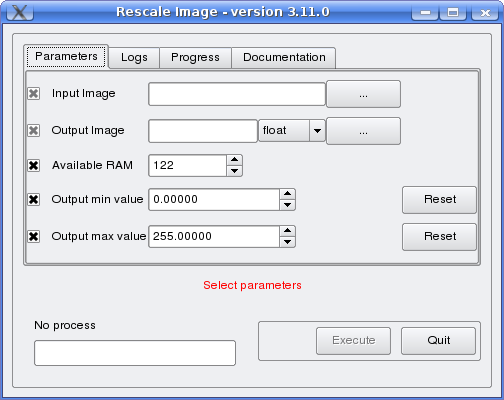
\includegraphics[width=0.6\textwidth]{../Art/QtImages/rescale_param.png}
  \itkcaption[GUI of the application Rescale, parameters tab]{Parameters tab in \application{Rescale} application.}
  \label{fig:rescaleParam}
\end{figure}

\begin{figure}[h]
  \center
  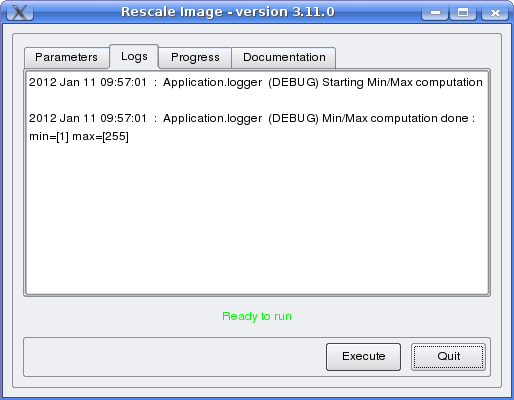
\includegraphics[width=0.6\textwidth]{../Art/QtImages/rescale_logs.png}
  \itkcaption[GUI of the application Rescale, logs tab]{Logs tab in \application{Rescale} application.}
  \label{fig:rescaleLogs}
\end{figure}

\begin{figure}[h]
  \center
  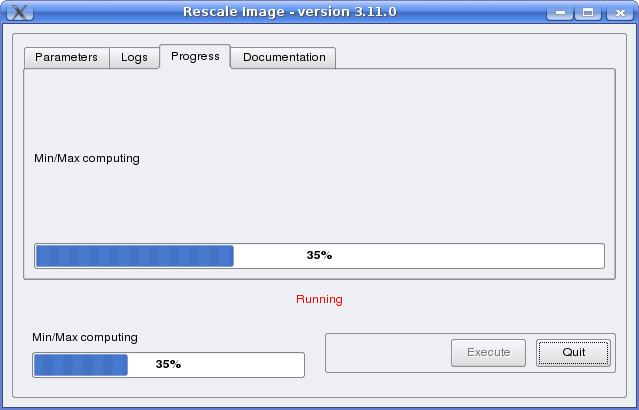
\includegraphics[width=0.6\textwidth]{../Art/QtImages/rescale_progress.png}
  \itkcaption[GUI of the application Rescale, progress tab]{Progress tab in \application{Rescale} application.}
  \label{fig:rescaleProgress}
\end{figure}

\begin{figure}[h]
  \center
  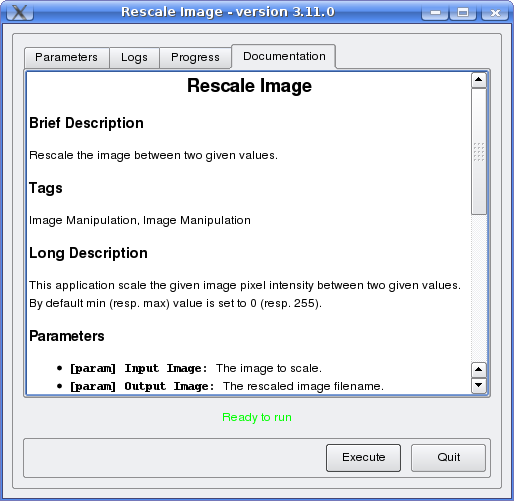
\includegraphics[width=0.6\textwidth]{../Art/QtImages/rescale_documentation.png}
  \itkcaption[GUI of the application Rescale, parameters tab]{Parameters tab in \application{Rescale} application.}
  \label{fig:rescaleDocumentation}
\end{figure}

\clearpage

\subsection{Using the Python interface}

The applications can also be accessed from Python, through a module named \verb?otbApplication?

On Unix systems it is typically available in the \verb?/usr/lib/otb/python? directory.
You may need to configure the environment variable \verb?PYTHONPATH? to include this directory
so that the module becomes available from an Python shell.

On Windows, you can install the \verb?otb-python? package, and the module will be available from
an OSGeo4W shell automatically.

In this module, two main classes can be manipulated :
\begin{itemize}
\item \verb?Registry?, which provides access to the list of available applications,
      and can create applications
\item \verb?Application?, the base class for all applications. This allows to interact with an application instance
      created by the \verb?Registry?
\end{itemize}

As for the command line and GUI launchers, the path to the application modules needs to
be properly set with the \verb?OTB_APPLICATION_PATH? environment variable.
The standard location on Unix systems is \verb?/usr/lib/otb/applications?.
On Windows, the applications are available in the \verb?otb-bin? OSGeo4W package, and
the environment is configured automatically so you don't need to tweak \verb?OTB_APPLICATION_PATH?.

Here is one example of how to use Python to run the \verb?Smoothing? application, changing the algorithm
at each iteration.

\begin{lstlisting}[language=python,breaklines=true,breakatwhitespace=true,frame = tb,framerule = 0.25pt,fontadjust,backgroundcolor={\color{listlightgray}},basicstyle = {\ttfamily\scriptsize},keywordstyle = {\ttfamily\color{listkeyword}\textbf},identifierstyle = {\ttfamily},commentstyle = {\ttfamily\color{listcomment}\textit},stringstyle = {\ttfamily},showstringspaces = false,showtabs = false,numbers = none,numbersep = 6pt, numberstyle={\ttfamily\color{listnumbers}},tabsize = 2]
#  Example on the use of the Smoothing application
#

# We will use sys.argv to retrieve arguments from the command line.
# Here, the script will accept an image file as first argument,
# and the basename of the output files, without extension.
from sys import argv

# The python module providing access to OTB applications is otbApplication
import otbApplication

# otbApplication.Registry can tell you what application are available
print "Available applications : "
print str( otbApplication.Registry.GetAvailableApplications() )

# Let's create the application with codename "Smoothing"
app = otbApplication.Registry.CreateApplication("Smoothing")

# We print the keys of all its parameter
print app.GetParametersKeys()

# First, we set the input image filename
app.SetParameterString("in", argv[1])

# The smoothing algorithm can be set with the "type" parameter key
# and can take 3 values : 'mean', 'gaussian', 'anidif'
for type in ['mean', 'gaussian', 'anidif']:

  print 'Running with ' + type + ' smoothing type'

  # Here we configure the smoothing algorithm
  app.SetParameterString("type", type)

  # Set the output filename, using the algorithm to differenciate the outputs
  app.SetParameterString("out", argv[2] + type + ".tif")

  # This will execute the application and save the output file
  app.ExecuteAndWriteOutput()

\end{lstlisting}



\subsection{Load/Save OTB-Applications parameters from/to file}

Since OTB 3.20, OTB applications parameters can be export/import to/from an XML
file using inxml/outxml parameters. Those parameters are available in all
applications.

An example is worth a thousand words

\begin{verbatim}
otbcli_BandMath -il input_image_1 input_image_2
                -exp "abs(im1b1 - im2b1)"
                -out output_image
                -outxml saved_applications_parameters.xml
\end{verbatim}

Then, you can run the applications with the same parameters using the output xml
file previously saved. For this, you have to use the inxml parameter:

\begin{verbatim}
otbcli_BandMath -inxml saved_applications_parameters.xml
\end{verbatim}

Note that you can also overload parameters from command line at the same time

\begin{verbatim}
otbcli_BandMath -inxml saved_applications_parameters.xml 
                -exp "(im1b1 - im2b1)"
\end{verbatim}

In this cas it will use as mathematical expression "(im1b1 - im2b1)" instead
of "abs(im1b1 - im2b1)".

Finally, you can also launch applications directly from the command-line launcher executable using
the inxml parameter without having to declare the application name. Use in this case:

\begin{verbatim}
otbApplicationLauncherCommandLine -inxml saved_applications_parameters.xml
\end{verbatim}
 
It will retrieve the application name and related parameters from the input xml
file and launch in this case the BandMath applications.

\subsection{Using OTB from QGIS}
\subsubsection{The processing toolbox}
OTB applications are available from QGIS. Use them from the processing toolbox,
which is accessible with Processing $\rightarrow$ Toolbox. Switch to "advanced interface"
in the bottom of the application widget and OTB applications will be there.

\begin{figure}[h]
  \center
  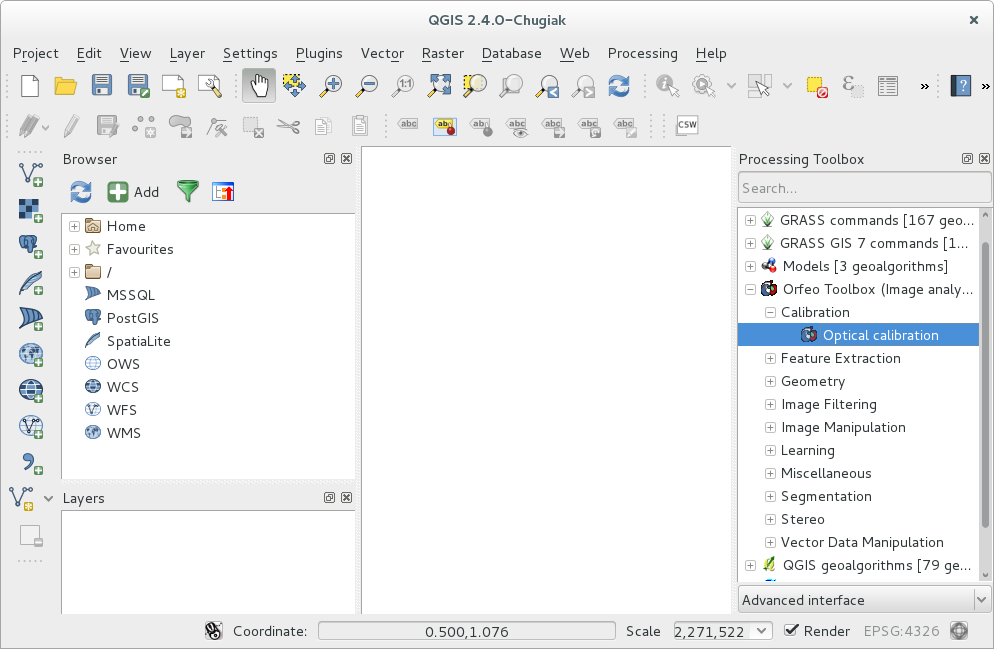
\includegraphics[width=0.6\textwidth]{../Art/QtImages/qgis-otb.png}
  \itkcaption[]{Processing toolbox in QGIS}
  \label{fig:otb-qgis}
\end{figure}

\subsubsection{Using a custom OTB}
If QGIS cannot find OTB, the "applications folder" and "binaries folder" can be
set from the settings in the Processing $\rightarrow$ Settings $\rightarrow$ "service provider".

\begin{figure}[h]
  \center
  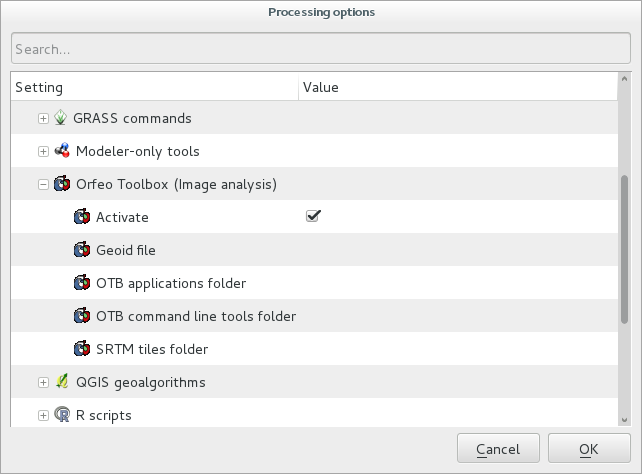
\includegraphics[width=0.6\textwidth]{../Art/QtImages/qgis-otb-settings.png}
  \itkcaption[]{Processing toolbox in QGIS}
  \label{fig:otb-qgis-settings}
\end{figure}

On some versions of QGIS, if an existing OTB installation is found, the
textfield settings will not be shown. To use a custom OTB instead of the
existing one, you will need to replace the otbcli,
otbgui and library files in QGIS installation directly.
